\chapter{Malicious URL detection and classification}\label{ch:malicious-url-detection-and-classification}

Whether you use the internet for business purpose or personal use, you can be a~victim of a~malware attack.
In order to prevent infection, security companies use tools like Domain Name System filtering to ensure, the users will not become victims of malware.
With large percentage of malicious \acrshort{url} links found on \say{good} domains and techniques like Domain Generation Algorithms, which does not require a~significant amount of sophistication while still being highly effective, it is impossible to capture all (or at least signifficant amount) vicious URLs without an automated system.
While there exists no simple rule, which would clearly distinguish between malicious and benign link, the machine learning system is necessary.

Detection of malicious URLs is effective when performed in real time, detects new URLs with high accuracy, and recognizes specific malicious activity type (e.g.\ phishing, spam, adware, drive-by-downloads etc.).
Nowadays, security vendors rely on filtering unencrypted DNS traffic based on signature detection (DNS firewall and blacklisting) to examine DNS queries and filter out known malicious domains.
This approach has its flaws.
Blocking is based on \textit{hostname}, which does not allow propper blocking of defaced URLs which contains both malicious and legitimate web pages.
Furthemore, in several years most of the DNS traffic will be encrypted, preventing any spying, spoofing or man-in-the-middle attacks, making the traditional entry-analyzing methods incapable to block malicious content~\cite{web:dns-encryption}.
There comes the ML solutions that can learn themselves on various types of datasets to identify malicious activity or anomalies within the web traffic.
Those datasets can be either bi-class (e.g.\ \say{bad} or \say{good} URLs) as presented in this paper or multi-class (e.g.\ malware, spyware, ransomware or fakenews, gambling sites and porn sites - depending on the requirements).
Other notable use of ML based URL classification is by proxy servers, which can provide filtration of complete URLs.
DNS and Proxy blocking can be performed both server and client side.

\section{Data}\label{sec:data}

The simplest way how to acquire data for URL classification would be to use some type of data which the system already collects.
Network monitoring is a common practice in all sorts of environments - therefore use of network monitor dump files, for example \textit{pcap} files would come in handy.
It is possible to obtain the full URLs from HTTP payloads together with other information like complete HTTP headers, the problem arises if the communication is encrypted by the SSL protocol.
The only information we can acquire from \textit{HTTPS captures} is hostname because almost every other usefull information is encrypted.
With HTTPS the path and query string of the URL is encrypted, while the hostname is visible inside the SSL \textit{handshake} as plain text.

The information like \textit{how long is the hostname registered} or \textit{website content} would be possible to get.
The methods used to acquire such information are very time and data consuming, while security system has to be fast and modest in data usage, therefore downloading web contents of every analyzed URL or calling additional query is not possible.

It would be best to use only the data we have available without additional information retrieval.
Furthemore the URLs are often constructed to deceive users (more information in the section~\ref{subsec:origins-of-malicious-urls}), therefore we want our features to be those exact characteristics.

\subsection{Origins of malicious URLs}\label{subsec:origins-of-malicious-urls}

While doing malicious URL classification, I have to mention, where do malicious URLs originate.
Some of the URLs are used for scam or phishing.
Such addresses are usually very similar to the original ones, e.g. \textit{goggle.com} instead of \textit{google.com} or \textit{arifrance.com} instead of \textit{airfrance.com} - this practise is called \textbf{typosquatting}~\cite{towards_data_science_phishing_url}.

\begin{align*}
    \underbrace{www}_\text{subdomain}
    \text{.}
    \underbrace{
        \overbrace{verylongdomainname}^\text{domain name}
        \text{.}
        \overbrace{academy}^\text{top-level domain}
    }_\text{root domain}
\end{align*}

Another similar practise known as \textbf{domain squatting} (also known as \textbf{cybersquatting}) consists in registering \textit{top-level domain} with \textit{second-level domain} belonging to some company.
Such domains are either sold to the company which owns the trademark or can be used with mischievous intentions.

\begin{quote}
    For example, the name of your company is \say{abcompany} and you register as abcompany.com.
    Then phishers can register abcompany.net, abcompany.org, abcompany.biz and they can use it for fraudulent purpose~\cite{towards_data_science_phishing_url}.
\end{quote}

Another approach is to generate addresses using Domain Generation Algorithm (DGA).
DGAs are used to produce a~large quantities of domains that are going to be used for communication to the malware's command and control servers~\cite{oracle_dga_scarfo}.
It is common practise for an DGA to generate 1000 domains which creates noise in the network.
Main objective of a~hacker is to register one of those addresses, which will become an active Command \& Control (C\&C) server.
Infected system then uses this address to communicate and receive commands from the attacker~\cite{what_are_dgas}.

Address created by DGA usually looks similar to this one: \textit{gwhhpnrfkdiedhga.ki} - pseudo-random set of characters, but other algorithms are more ingenious - combining established techniques with word dictionaries (e.g. \textit{101paypal-login.in}).

DGA domain detection can be complicated.
Some techniques use Shannon entropy or n-grams, but those are most effective in recognising pseudo-random addresses.
To recognise the other ones, we need different approach - machine learning algorithm combining above-mentioned techniques~\cite{building_dga_classifier,what_are_dgas,entropy_dns}.

\subsection{Datasets}\label{subsec:datasets}

For classifier training which will distinguish between malicious and harmless (benign) URLs, the dataset with URL and class (with labels \textit{good} and \textit{bad}) will be needed.
Probably the largest available dataset is available from University of California San Diego at the \url{http://www.sysnet.ucsd.edu/projects/url/}.
The data was made available as part of a~research project, containing data from 120 days and each observation has approximately \num{3200000} features.
The target variable contains \( 1 \) if it is a~malicious website and \( -1 \) otherwise.
Large dataset like this one would be ideal.
Unfortunatelly, the data are already in a~form of matrices of features, therefore feature extraction is not possible, making dataset unsuitable for this study.

To be able to produce vectorizer and feature matrix, raw data are necessary - URL in its raw string form, with label denoting class affiliation.
Datasets meeting those conditions can be found quite easily, although some of them are rather specific, labeling malicious URLs cording to the type of exploitation - malware, spyware, ransomware, etc.
Those sets can be used, but even more suitable ones can be found.

In the practical example is used a~combined set of URLs from sources mentioned in the table~\ref{table:dataset-information} and table~\ref{table:dataset-statistics}.
\textbf{Hosts} is a~repository which consolidates reputable \textit{hosts} files, creating list of potentinally unwanted websites focusing on fakenews, gambling, porn and general malicious URLs.
The Kaggle.com is website offering ML challenges and datasets for general public, all supported by the Kaggle community.

For the classifiers' training a~\textbf{balanced} dataset was generated, containing total of \num{125000} URLs - \( 50\% \) malign, \( 50\% \) benign, with minimal URL length of \( 5 \) characters, average URL length of \( 45 \) characters, maximum URL length of \num{2307} characters, mode of \( 31 \) and median of \( 35 \) characters.

\begin{table}[htb]
    \centering

    {\small
    \begin{tabular}{lll}
        \toprule
        Dataset & Download date         & URL \\
        \midrule
        Kaggle  & 28th Semptember 2018  & \url{https://www.kaggle.com/antonyj453/urldataset#data.csv} \\
        Hosts   & 12th March 2019       & \url{http://sbc.io/hosts/alternates/fakenews-gambling-porn/hosts} \\
        \bottomrule
    \end{tabular}
    }

    \caption{Information about datasets (name, download date and download URL)}
    \label{table:dataset-information}
\end{table}
\FloatBarrier

\begin{table}[htb]
    \centering

    {\small
    \begin{tabular}{lrrrcrccc}
        \toprule
                    & \multicolumn{3}{c}{Number of samples}         & \multicolumn{5}{c}{Length of URL} \\ \cmidrule(lr){2-4} \cmidrule(lr){5-9}
        Dataset     & Total         & Malicious     & Benign        & Minimal & Maximal     & Average   & Mode      & Median \\
        \midrule
        Kaggle      & \num{411247} & \( 18\% \)    & \( 82\% \)     & \( 6 \) & \num{2307}  & \( 48 \)  & \( 31 \)  & \( 41 \) \\
        Hosts       & \num{55575}  & \( 100\% \)   & \( 0\% \)      & \( 5 \) & \( 93 \)    & \( 18 \)  & \( 17 \)  & \( 18 \) \\
        \bottomrule
    \end{tabular}
    }

    \caption{Information about datasets (name, number of samples and URL statistics)}
    \label{table:dataset-statistics}
\end{table}
\FloatBarrier

The final training dataset is a~\textit{csv} file in the format as in the table~\ref{table:dataset-example}, with the header \textit{url, label}.
For the testing purposes, four other dataset were made.
Those sets are made in order to simulate real-world network traffic, where data are strongly biased.
The first set is unbiased, the second one consists of ten times as much benign as malicious samples.
The third set has hundred times and the fourth has thousand times more benign samples.
In the concrete numbers:
\begin{enumerate}
    \item \( 300 \) malign samples to \num{300} benign samples;
    \item \( 300 \) malign samples to \num{3000} benign samples;
    \item \( 300 \) malign samples to \num{30000} benign samples (refered to as \say{set with \( 1:100 \) ratio});
    \item \( 300 \) malign samples to \num{300000} benign samples.
\end{enumerate}

\begin{table}[htb]
    \centering

    \resizebox{\textwidth}{!}{%
    \begin{tabular}{ll}
        \toprule
        URL & Label \\
        \midrule
        \nolinkurl{https://www.kino24.kz/blog/engine/modules/plugin/source.php?id=} & bad \\
        \nolinkurl{https://www.warcraft-lich-king.ru/wp-admin/present.php?origin=lobs&amp;session=NzEwMTU2MDkwNDM0Nzk} & bad \\
        \nolinkurl{https://phxfw.wordpress.com/2011/11/19/phxfws-own-to-judge-miss-arizona-teen-pageants/} & good \\
        \nolinkurl{http://www.vertor.com/torrents/117148/Macy-Gray-The-Very-Best-Of-Macy-Gray} & good \\
        \nolinkurl{https://www.mycomicshop.com/search?TID=174061} & good \\
        \bottomrule
    \end{tabular}%
    }

    \caption{Dataset example}
    \label{table:dataset-example}
\end{table}
\FloatBarrier

The development data were created from the dataset with \( 1:100 \) ratio by spliting the set into 80\% \textit{test} and 20\% \textit{dev} set.

\section{Text feature extraction}\label{sec:text-feature-extraction}

Text feature extraction is a~process of tokenizing, counting and normalizing string data to be fed to the machine learning algorithms.
In general, only a~few groups of features for URL classification are commonly used.

\begin{itemize}
    \item \textbf{URL-Based Features} are extracted from URL\@.
    Examples are \textit{total length of address}, \textit{number of digits in URL}, \textit{legitimate name of brand in subdomain} or \textit{number of subdomains}.

    \item \textbf{Domain-Based Features} consist of information about domain registrant and domain itself, e.g. \textit{how many days passed since the domain was registered} or if \textit{is the registrant name hidden}.

    \item \textbf{Page-Based Features} are harder to obtain, then the others.
    Such features are obtainable from tools like \textbf{Google Analytics} - \textit{average visit duration}, \textit{number of pages visited}, etc.
    In most cases, PageRank is the easiest metric to get.

    \item \textbf{Content-Based Features} are collectable with technique called \textbf{web scraping}.
    Data are extracted from website and analysis is performed.
\end{itemize}

The paper focuses on the use of \textit{URL-based} features (specifically \textit{word occurences}) - while the dataset does contain already blocked and inactive URLs, there is no possibility to extract \textit{domain-based}, \textit{page-based} or \textit{content-based} features.
At the same time, the use of \textit{URL-based} features is potentially safer (there is no need to download anything from the website) and represents an interesting challenge to classify a~URL with minimal memory and performance requirements.

The whitepaper \say{Heuristic-based Approach for Phishing Site Detection Using URL Features} published in 2015 describes the Korean team's solution for phishing site detection using URL features~\cite{Lee2015HeuristicbasedAF}.
The team presents 26 features which are used in the detection mechanism they created.

First group of features is related to Google search engine suggestions.
First three features are based on similarity of primary domain, subdomain and a~path to Google suggestions.
The other three features checks whether searched term (domain, subdomain and path) is presented in a~whitelist.
Levenshtein distance between the two terms is calculated.
If a~search term is similar to the suggested one, then it is more likely to be marked as a~suspicious, because that site may be used as a~trap when user misspells a~word/address~\cite{Lee2015HeuristicbasedAF}.
If the Levenshtein distance equals to zero (both terms are the same), then domain is added into the trustworthy whitelist, such site is probably legitimate.

The are three features in the second group, which are extracted through page ranking.
PageRank is an algorithm which offers a~way of measuring the importance of a~website.
Malicious websites usually have a~very low page rank value because such sites are not visited by many people and they exists only for a~short time~\cite{Lee2015HeuristicbasedAF}.

Third group is about analysing the structure of URL address and its patterns.
URL rarely contains some special characters and legitimate sites usually have one \say{top-level domain}.
Therefore many TLDs can signify a~fraudulent site.

In the next group URL property values are checked.
Temporary malicious URLs often does not use HTTPS protocol and does not have DNS or WHOIS record.

Lastly length of a~subdomain is calculated and phishing terms in the URL are checked.

In the end the research team compared several algorithms on the sample of \num{6000} URLs. In the conclusion they evaluate \say{random forest} classifier as the best, for their case.
Unfortunately model parameters are not mentioned, and their training and testing data are not available, therefore we are not able to reproduce their outcome.

\subsection{Tokenization}\label{subsec:tokenization}

In our case, string tokenization of URL is done with \textit{wordninja} module, which works by modeling the distribution of the output, assuming all words are independently distributed~\cite{stackoverflow:tokenizer}.
In order to properly tokenize continuous chain of words (also known as \textit{string} without spaces), we need to have a~list of words sorted from high to low by frequency.
The relative frequency of words in a~given language can be calculated for example from Wikipedia articles dataset.
For each word in the frequency set, the \say{word-cost} is calculated with the equation (\ref{eq:word-cost}), where \( N \) is the total number of words and \( k \in \{ 1, 2, \ldots, N \} \) is the rank of word in dataset.

\begin{align}
    wordcost = \log\left( k \cdot \log(N) \right) \label{eq:word-cost}
\end{align}

Let \( s \) to be an URL\@.
The dynamic programming is used to infer the position of the spaces.
As the first step, the \textit{cost array} is build, containing one number for each character in the original string \( s \).
This array is created by iterating over characters in \( s \), calculating the minimum cost of the first \( i \) characters, based on \textit{word-cost}, value of charater at the position \( i - 1 \) and every possible contiguous subsequence of characters with common upper border, given by the index \( i \).

After that, the \textit{cost array} is backtracked to recover the minimal-cost string.
Array of characters, represented by \( s \) is iterated once again, but backwards.
The minimum cost of the set of characters ending with \( j := length(s) \) is retrieved (that is why the \textit{cost array} was needed), together with number of characters \( l \), which make up the minimum value.
The interval of characters from index \( j - l \) till \( j \) is one of the words, we were looking for.
Now a~new ending character is set to \( j = j - l \) and \textit{backtracking} continues until \( j \) is zero.

The advantage of this solution is that the implementation consumes a~linear amount of time and memory~\cite{stackoverflow:tokenizer}.
The disadvantage, on the other hand, is the necessity to have the corpus of words sorted by relative word frequency similar to what will the tokenizer actually encounter (e.g.\ the correct language), otherwise the results will be very bad~\cite{stackoverflow:tokenizer}.
Implementation of the algorithm is available at the appendix~\ref{ch:url-tokenizer}.

In the end, the four special tokens are removed - TLD \textit{com}, subdomain \textit{www} and protocols \textit{http}, \textit{https}.
They are present to such an extent that it would be very inappropriate to draw conclusions based on their presence.

\begin{align*}
    \text{brownfoxjumpsoverdog} &\rightarrow \left( \text{brown}, \text{fox}, \text{jumps}, \text{over}, \text{dog} \right) \\
    \text{0ZStYTgvFu1U85XxLeE9} &\rightarrow \left( \text{0}, \text{z}, \text{sty}, \text{tgv}, \text{fu}, \text{1}, \text{u}, \text{85}, \text{xx}, \text{lee}, \text{9} \right)
\end{align*}

\subsection{Vectorization}\label{subsec:vectorization}

For counting and normalizing I am going to use \textit{scikit-learn's} TF-IDF vectorizer.
TF-IDF stands for \textit{term-frequency times inverse document-frequency}, it is a~statistical measure to evaluate the importance of a~word to document in a~corpus~(\ref{eq:tf-idf}).
In the equation, \( \tf{t, d} \) is how many times that term \( t \) occurs in a~document \( d \) - this is called \textit{raw count}.
By default normalized term-frequency is used by \textit{scikit-learn}~(\ref{eq:tf}).
There are other options that can be used like boolean frequency where \( \tf{t, d} = 1 \) if \( t \) occurs in given \( d \) and \( 0 \) otherwise, or logarithmically scaled frequency where \( \tf{t, d} \) is replaced with \( 1 + \log(\tf{t, d}) \).

\begin{align}
    \tf{t, d} &= \frac{\text{number of times} \: t \: \text{appears in} \: d}{\text{total number of terms in} \: d} \label{eq:tf} \\
    \tfidf{t, d} &= \tf{t, d} \times \idf{t} \label{eq:tf-idf} \\
    \idf{t} &= \log{\frac{1 + n}{1 + \df{t}}} + 1 \label{eq:idf}
\end{align}

Inverse document-frequency is computed as in the equation~(\ref{eq:idf}) where \( n \) is is the total number of documents in the corpus.
The function \( \df{t} \) is the number of documents in the corpus that contain term \( t \).
The TF-IDF vectors are then normalized by the Euclidean (L2) norm~(\ref{eq:l2-norm}).

\begin{align}
    v_{norm} = \frac{v}{||v||_2} = \frac{v}{\sqrt{v{_1}^2 +  v{_2}^2 + \dots + v{_n}^2}} \label{eq:l2-norm}
\end{align}

As can be seen, \textit{TfidfVectorizer} has two usefull properties:
\begin{enumerate*}[label=(\roman*)]
    \item it lowers the weight of common words,
    \item applies Euclidean normalization after computing the TF-IDF representation.
\end{enumerate*}

Implementation of scikit learn TF-IDF vectorizer consists of two parts.
As mentioned in the section~\ref{subsec:tokenization}, each URL in corpus tis splitted into individual words - tokens.
The \textbf{CountVectorizer} then converts a~this collection of words to a~matrix of token counts (\ref{eq:count-vectorizer}).

\begin{equation}
    \label{eq:count-vectorizer}
    \begin{matrix}
        \text{This is the first sentence.} \\
        \text{This sentence is the second sentence.} \\
        \text{And this is the third one.} \\
        \text{Is this the first sentence?}
    \end{matrix}
    \Rightarrow
    \begin{matrix}
        \text{and} \\ \text{sentence} \\ \text{first} \\ \text{is} \\ \text{one} \\ \text{second} \\ \text{the} \\ \text{third} \\ \text{this}
    \end{matrix}
    \Rightarrow
    \begin{bmatrix}
        0 & 1 & 1 & 1 & 0 & 0 & 1 & 0 & 1 \\
        0 & 2 & 0 & 1 & 0 & 1 & 1 & 0 & 1 \\
        1 & 0 & 0 & 1 & 1 & 0 & 1 & 1 & 1 \\
        0 & 1 & 1 & 1 & 0 & 0 & 1 & 0 & 1
    \end{bmatrix}
\end{equation}

An encoded matrix is returned with a~length of the entire vocabulary and an integer count for the number of times each word appeared in the collection.

In our case (word occurences in URLs), this matrix is extremely sparse (most of the elements in matrix is \( 0 \)).
The total count of features in the presented dataset is around \num{1150000}, while each URL has only a~few tokens (in the order of units).

The other constituent part of TF-IDF vectorizer is TF-IDF transformer.
This transformer converts a~count matrix to a~normalized \textit{term-frequency} or \textit{term-frequency times inverse document-frequency} portrayal.
We are going to prefer tf-idf instead of the raw frequencies of occurrence of a~token, because the objective is to scale down the importance of words that appear more frequently in a~given corpus.
Informative function of such tokens is (verifiable by experience) lower than descriptive value of words that occure less often in the training set.

Eucledian rescaling means that the each representation of URL has L2 norm equal to \( 1 \), therefore length of URL (the number of tokens) does not change the vectorized representation~\cite{web:stackexchange_l2norm}.

The vector of token frequencies for a~given URL is called a~sample~\cite{scikit-learn}.
Process of counting and normalizing is called vectorization, the result is \textbf{Bag of Words} representation.
\textbf{Bag of Words} is a~strategy of describing a~document (in our case an URL) by word occurences ignoring the relative position of the words~\cite{scikit-learn}.

\newpage
\section{Classifiers}\label{sec:classifiers}

There are many options which classifier to choose for text classification.
To name a~few supervised learning options~\cite{web:popular-text-classifiers}:

\begin{itemize}
    \item \textbf{Support Vector Machines},
    \item \textbf{Logistic Regression},
    \item \textbf{Naive Bayes},
    \item Neural Networks,
    \item Hidden Markov models,
    \item Decision Trees,
    \item Random Forests,
    \item Boosting and Bagging algorithms,
    \item k-Nearest Neighbour algorithm.
\end{itemize}

Each one of them has advantages and disadvantages, which determine how and when can be those methods used.
Point of this work is not to train algorithm with high classification success rate.
The chosen classifiers were chosen in order to present a~wide scale of possible solutions with relatively high classification rate without need to \say{tweak} model hyperparameters.

The problem, the paper faces, is text binary classification with large sparse matrix as an input.
With respect to those criteria, I chose three suitable classifiers - SVM with stochastic gradient descent method, logistic regression and multinomial Naive Bayes.

During the research, I tried others, like decision trees and random forests, but those two generally do not work well with sparse data.
There are some exceptions and although DT and RF can work well with sparse data if specific parameters (e.g.\ number of trees and number of features evaluated at each split decision) are set in a~reasonable way, they were labeled as \say{not suitable} for this task.

KNN algorithm is used to classify instance by finding the \( k \) nearest matches in training data and then using the label of closest matches to predict the category.
Traditionally, distance such as euclidean is used to find the closest match~\cite{web:knn-text-classification}.
The method can use several algorithm to search for points in k-dimesional space like \textit{k-d tree} or \textit{ball tree}, unfortunatelly the brute-force search is used by \textit{scikit-learn's} implementation of algorithm, which is memory inefficient and raises MemoryError on my computer for the task, not being able to complete training.

\subsection{Stochastic gradient descent}\label{subsec:stochastic-gradient-descent}

Stochastic Gradient Descent is a~popular optimization technique, which can be used with many learning algorithms.
\textit{SGDClassifier} is a~linear classifier (linear SVM) that uses Stochastic Gradient Descent for training.
In addition it requires less memory and allows incremental (online) learning~\cite{scikit-learn}.
Support vector machines are effective in high dimensional spaces and use only a~subset of training points in the decision function (called support vectors), so it is memory efficient~\cite{scikit-learn}.

Gradient Descent is an iterative method, used to find the values of the parameters of a~function that minimizes the cost function as much as possible.
The difference between Gradient Descent optimization and SGD is that the second one uses only a~few \textit{randomly} selected samples instead of the whole data set for each iteration.
Using the whole dataset is useful for getting to the minima in a~less noisy or less random manner, but when datasets are humongous (very large), it becomes computationally very expensive~\cite{web:stochastic-gradient-descent}.

Disadvantage is that SGD requires a~number of hyperparameters and is sensitive to feature scaling~\cite{scikit-learn}.
The \textit{scikit-learn} implementation requires \verb|loss="log"| parameter to be used in order to enable the \verb|predict_proba| method, which gives a~vector of probability estimates \( P(y{\mid}x) \) per sample \( x \).
Method \verb|predict_proba| is required by LIME framework (introduced in chapter~\ref{ch:model-analysis}).
The SGD classifier supports multi-class classification by combining multiple binary classifiers into one.

The model is given a~set of training examples \( (x_1, y_1), \ldots, (x_n, y_n) \) where \( x_i \in \mathbf{R}^m \) and \( y_i \in \{-1,1\} \)~\cite{scikit-learn}.
The goal is to figure out a~linear scoring function \( f(x) = w^T x + b \) with parameters \( w \in \mathbf{R}^m \) and intercept \( b \in \mathbf{R} \)~\cite{scikit-learn}.
The prediction is made by looking at the sign of \( f(x) \).
Model parameters are found by minimizing the regularized training error~(\ref{eq:sgd-error}), where \( L \) is a~loss function that measures model fit, \( R \) is a~regularization term that penalizes model complexity and \( \alpha > 0\) is a~non-negative hyperparameter~\cite{scikit-learn}.

\begin{align}
    E(w,b) = \frac{1}{n}\sum_{i=1}^{n} L(y_i, f(x_i)) + \alpha R(w) \label{eq:sgd-error}
\end{align}

Model in the following example uses \textit{logistic regression} as a~loss function \( L \) and the regularization term is the default one (L2 norm) \( R(w) := \frac{1}{2} \sum_{i=1}^{n} w_i^2 \).

\subsection{Logistic regression}\label{subsec:logistic-regression}

Logistic regression is a~linear, naturally interprettable model for classification and is an extension of the linear regression model for classification problems.
\textit{Scikit-learn's} implementation can fit binary, One-vs-Rest, or multinomial logistic regression~\cite{scikit-learn}.

Input values \( \mathbf{x} \) are linearly combined using weights \( \mathbf{\beta} \) to predict an output value \( y \).

\begin{align}
    y = \frac{exp(\beta_0 + \beta_1 \cdot x_1 + \ldots + \beta_k \cdot x_k)}{1 + exp(\beta_0 + \beta_1 \cdot x_1 + \ldots + \beta_k \cdot x_k)}
\end{align}

The \( \beta_0 \) is the bias, \( \beta_1, \ldots, \beta_k \) where \( k \in \{ 1, 2, \ldots \} \) are the coefficient that must be estimated from the training data.
This is done using \textit{maximum-likelihood estimation} - a~minimization algorithm which obtains the parameter estimates by finding the parameter values that maximize the likelihood function~(\ref{eq:logistic-function})~\cite{web:logistic-regression}.

\begin{align}
    \text{lf}(\mathbf{x})=\frac{1}{1+exp(-\mathbf{x})} \label{eq:logistic-function}
\end{align}

Logistic regression requires for data to meet several requirements~\cite{web:logistic-regression}:

\begin{itemize}
    \item binary output variable,
    \item noiseless data (since the method assumes no error in the output variable),
    \item absence of correlated inputs (the model can overfit if multiple highly-correlated inputs are present).
\end{itemize}

If all assumptions of the linear regression model are met by the data, there is a~guarantee to find optimal weights~\cite{web:logistic-regression}.

The disadvantages are oversimplifying resulting in \say{not that good} predictive performance and risk of \textit{complete separation}, occuring in the case in which there is a~feature that would perfectly separate the two classes (weight for that feature would not converge), although there is no need for machine learning in that scenario.

\subsection{Multinomial Naive Bayes}\label{subsec:multinomial-naive-bayes}

Naive Bayes is a~set of methods based on applying Bayes' theorem.

\begin{align}
    P(y \mid x_1, \dots, x_n) = \frac{P(y) P(x_1, \dots x_n \mid y)}{P(x_1, \dots, x_n)}
\end{align}

To reduce the number of parameters, we make the \say{naive} Bayes \textit{conditional independence assumption}.
We assume that attribute values are independent of each other given the class~\cite{book:introduction-to-information-retrieval}.

\begin{align}
    P(x_i | y, x_1, \dots, x_{i-1}, x_{i+1}, \dots, x_n) = P(x_i | y)
\end{align}

Multinomial distribution is a~generalization of the binomial distribution.
Multinomial Naive Bayes is algorithm implemented for multinomially distributed data, suitable for classification with discrete features (word counts for text classification).

Although Bayes method is decent classifier, it is a~bad probability estimator, therefore the probability outputs from \verb|predict_proba| are not accurate.
Naive Bayes algorithms are mostly used in sentiment analysis, spam filtering or recommendation systems.
For document classification problem (whether a~document belongs to the category of music, technology, sport,\ldots), Multinomial Naive Bayes is mostly used.

The data distribution is parametrized by vectors \( \theta_y = (\theta_{y1},\ldots,\theta_{yn}) \) for every class \( y \) where \( n \) is the size of the vocabulary and \( \theta_{yi} \) is the probability \( P(x_i \mid y) \) of feature \( i \) appearing in a~sample belonging to class \( y \)~\cite{scikit-learn}.
The parameters \( \theta_y \) are estimated by the equation (\ref{eq:smoothed-maximum-likelihood}).

\begin{align}
    \hat{\theta}_{yi} = \frac{ N_{yi} + \alpha}{N_y + \alpha n} \label{eq:smoothed-maximum-likelihood}
\end{align}

The number of how many times the feature \( i \) appears in a~sample of class \( y \) in the training set \( T \) is denoted by \( N_{yi} = \sum_{x \in T} x_i \)~\cite{scikit-learn}.
The \( N_{y} = \sum_{i=1}^{n} N_{yi} \) is the total count of all features for class \( y \)~\cite{scikit-learn}.
The smoothing coeficient \( \alpha \ge 0 \) accounts for features not present in the learning samples and prevents zero probabilities in further computations~\cite{scikit-learn}.

Other types are Bernoulli and Gaussian Naive Bayes.
The Bernoulli Naive Bayes classifier assumes that all our features are binary, therefore not suitable for text classification with tf-idf features.
Gaussian Naive Bayes (\ref{eq:gaussian-bayes}) is used in cases when all features are continuous (assumption of the normal distribution) - not made for cases where features can be represent in terms of their occurrences (text classification)~\cite{web:naive-bayes-differences}.

\begin{align}
    P(x_i \mid y) = \frac{1}{\sqrt{2\pi\sigma^2_y}} \exp\left(-\frac{(x_i - \mu_y)^2}{2\sigma^2_y}\right) \label{eq:gaussian-bayes}
\end{align}

\newpage
\section{Evaluation}\label{sec:evaluation}

The main metrics used for evaluation are \textit{precision}, \textit{recall} and \textit{f1-score};
where TP = True positive, FP = False positive, FN = False negative and TN = True negative.

\begin{align}
    precision &= \dfrac{TP}{TP + FP} \\
    recall &= \dfrac{TP}{TP + FN} \\
    F1 &= 2 \cdot \dfrac{precision \cdot recall}{precision + recall}
\end{align}

The \textit{precision} is the ability of the classifier not to label as positive a~sample that is negative.
The \textit{recall} is the ability of the classifier to find all the positive samples.
The F1-score can be interpreted as a~weighted average of the precision and recall, where the score reaches its best value at 1 and worst score at 0.

In the real world, malicious traffic is always hidden in much larger set of daily, benign data flow.
The question, how the trained classifiers perform on those heavily biased data sets arises.
Dataset bias is a~problem beyond the scope of this paper, yet, let me examine consequences of bias for URL classification.

Models were trained using \textit{scikit-learn's} default parameters, with the currated balanced dataset.
The accuracy and precision, recall and F1-score for malicious classification are in the table~\ref{table:combined-report}, \textit{support} is the number of samples from the testing dataset that lie in that particular class.
The data for the report in the table~\ref{table:combined-report} is the testing part (the 80\%) from the set with \( 1:100 \) ratio, the same data were used to create ROC curve in the figure~\ref{fig:roc}.
The ROC curve is a~performance measurement for classification at various thresholds settings, giving the information how much is model able to distinguish between classes.

\begin{table}[htb]
    \centering

    \begin{tabular}{lcccc}
        \toprule
        Classifier & Precision & Recall & F1-score & Support \\
        \midrule
        SGD & 0.11 & 0.92 & 0.19 & 239 \\
        LRC & 0.15 & 0.97 & 0.26 & 239 \\
        MNB & 0.11 & 0.97 & 0.19 & 239 \\
        \bottomrule
    \end{tabular}

    \caption{Combined classification report for Stochastic gradient descent (SGD), Logistic regression (LRC) and Multinomial Naive Bayes (MNB) classifier with the default threshold \(= 0.5 \) for class \textit{bad}}
    \label{table:combined-report}
\end{table}
\FloatBarrier

\begin{figure}[htb]
    \centering
    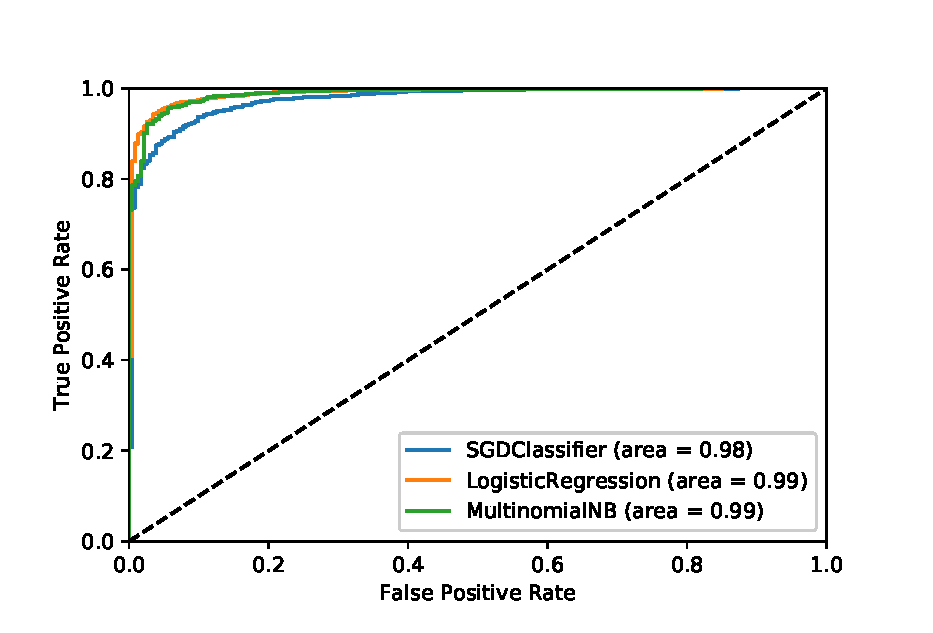
\includegraphics[width=0.7\textwidth]{imgs/roc.eps}
    \caption{Receiver operating characteristic (ROC) curve for given classifiers}
    \label{fig:roc}
\end{figure}
\FloatBarrier

The \textit{scikit-learn} use a~default threshold of \( 0.5 \) for binary classifications.
From the development part (the 20\%) from the set with \( 1:100 \) ratio, the figures~\ref{fig:sgd-threshold},~\ref{fig:lrc-threshold} and~\ref{fig:mnb-threshold} were created, in order to view precision, recall and F1-score at various thresholds.
Therefore the ideal threshold for particular data and classifier combination can be determined.

\begin{figure}[htb]
    \centering
    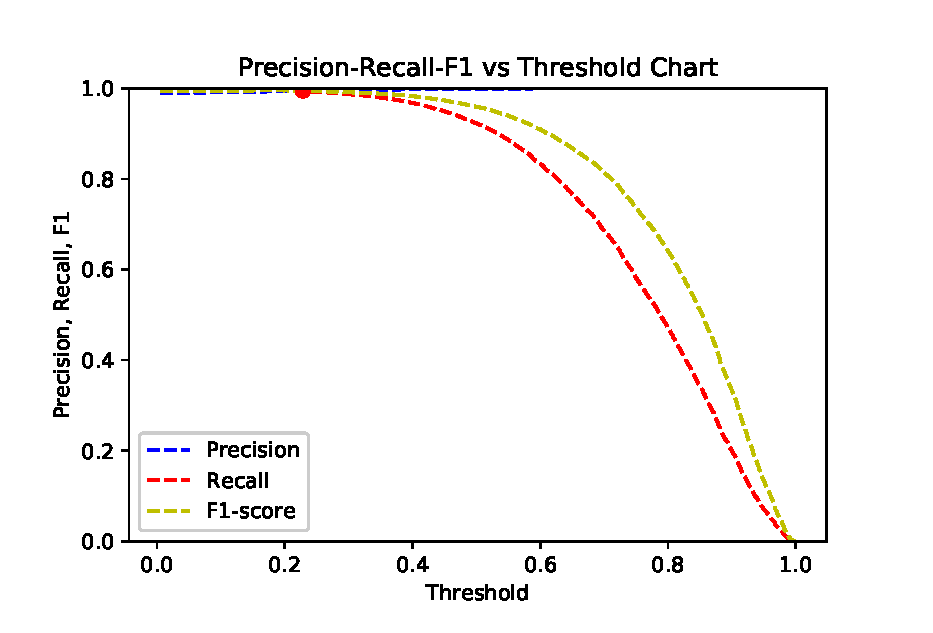
\includegraphics[width=0.7\textwidth]{imgs/SGDClassifier-prec-rec-thresh.eps}
    \caption{Precision, recall and F1-score at various thresholds for SGD classifier}
    \label{fig:sgd-threshold}
\end{figure}
\FloatBarrier

\begin{figure}[htb]
    \centering
    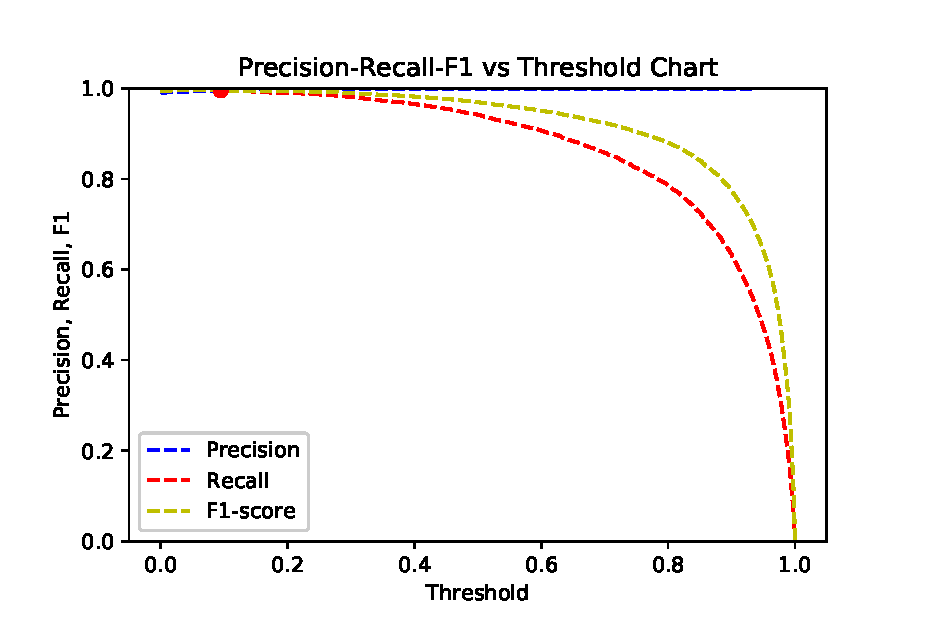
\includegraphics[width=0.7\textwidth]{imgs/LogisticRegression-prec-rec-thresh.eps}
    \caption{Precision, recall and F1-score at various thresholds for Logistic regression classifier}
    \label{fig:lrc-threshold}
\end{figure}
\FloatBarrier

\begin{figure}[htb]
    \centering
    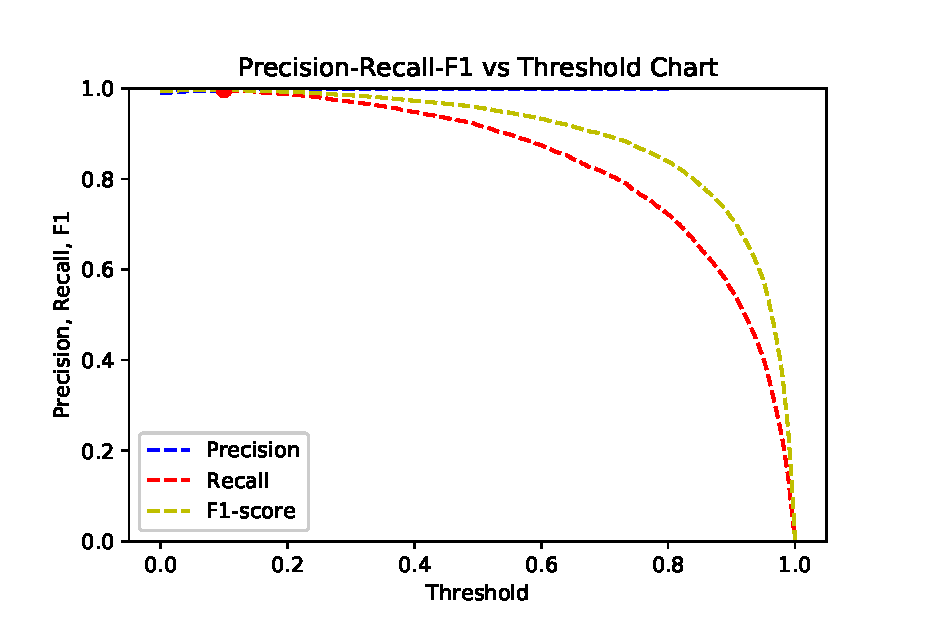
\includegraphics[width=0.7\textwidth]{imgs/MultinomialNB-prec-rec-thresh.eps}
    \caption{Precision, recall and F1-score at various thresholds for Multinomial NB classifier}
    \label{fig:mnb-threshold}
\end{figure}
\FloatBarrier

Now we know that the default threshold (\( 0.5 \)) is not optimal, therefore the new classification report with optimal thresholds is generated.

\begin{table}[htb]
    \centering

    \begin{tabular}{lccccc}
        \toprule
        Classifier & Threshold & Precision & Recall & F1-score & Support \\
        \midrule
        SGD & 0.217 & 0.55 & 0.53 & 0.54 & 239 \\
        LRC & 0.098 & 0.65 & 0.64 & 0.64 & 239 \\
        MNB & 0.110 & 0.67 & 0.68 & 0.67 & 239 \\
        \bottomrule
    \end{tabular}

    \caption{Combined classification report for Stochastic gradient descent (SGD), Logistic regression (LRC) and Multinomial Naive Bayes (MNB) classifier with the optimal thresholds for malicious class}
    \label{table:combined-report-optimal}
\end{table}
\FloatBarrier

For the last evaluation test case the four testing sets, each one with different distribution ratio, were used.
The results are in the figure~\ref{fig:ratios}.
The results shows the higher the ratio, the lower the optimal threshold and lower the F1-score.

\begin{figure}[htb]
    \centering
    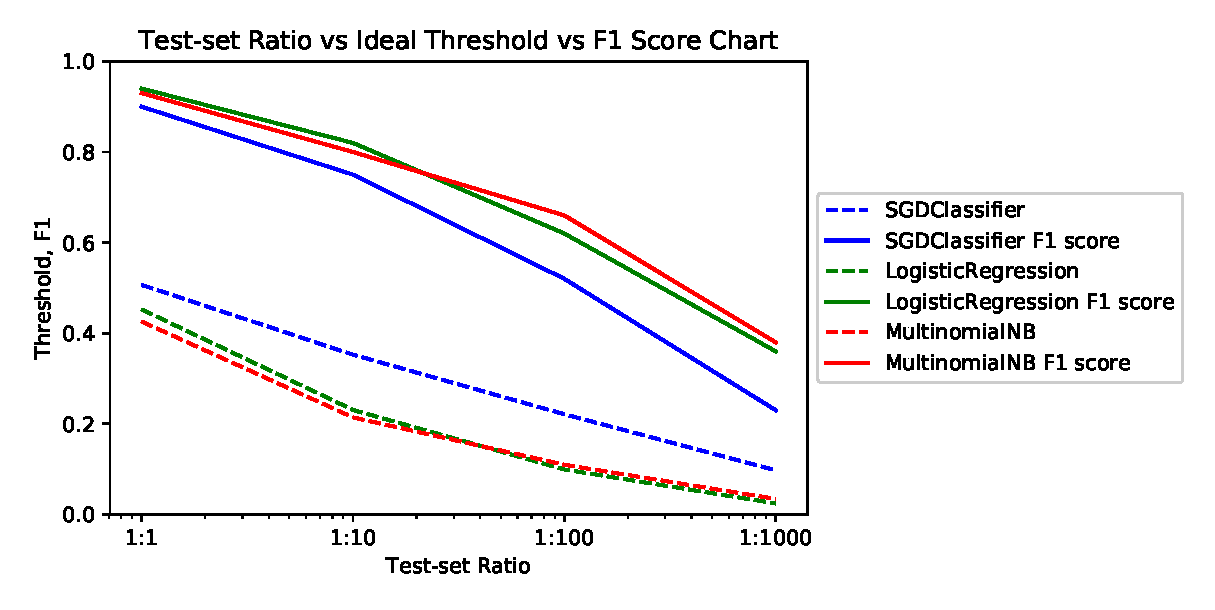
\includegraphics[width=0.9\textwidth]{imgs/ratios.eps}
    \caption{Ideal classification thresholds vs test set ratios vs F1-score for malicious class}
    \label{fig:ratios}
\end{figure}
\FloatBarrier


